Containerisierung ist ein Virtualisierungsverfahren, bei dem Anwendungen 
zusammen mit allen erforderlichen Abhängigkeiten in isolierten 
Laufzeitumgebungen bereitgestellt werden. Diese Umgebungen werden als 
\textbf{Container} bezeichnet \cite{docker_overview}.

Anders als klassische virtuelle Maschinen emulieren Container nicht die 
vollständige Hardware-Schicht, sondern teilen sich den Kernel des 
Host-Systems. Das führt zu deutlich geringerem Ressourcenverbrauch und 
kürzeren Startzeiten \cite{redhat_container}. 
Abbildung~\ref{fig:container-vs-vm} zeigt diesen Unterschied.

\begin{figure}[H]
    \centering
    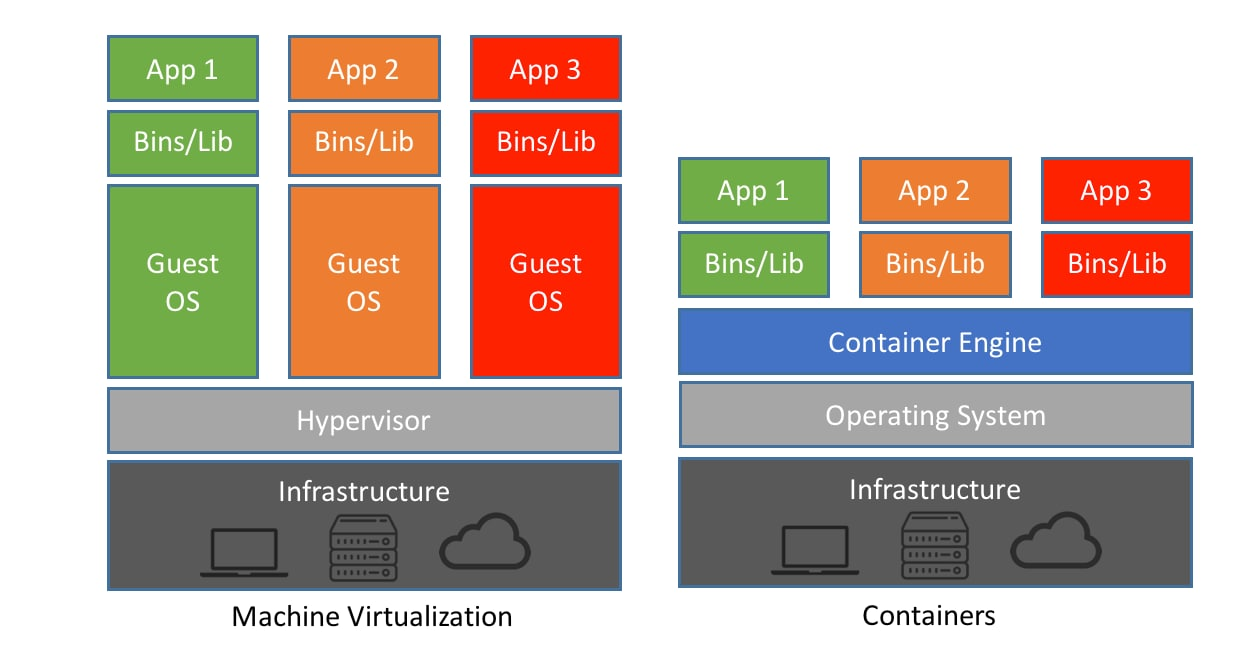
\includegraphics[width=0.8\textwidth]{pics/container-vs-vm-inline1_tcm19-82163.jpg}
    \caption{Vergleich zwischen Containern und virtuellen Maschinen}
    \label{fig:container-vs-vm}
\end{figure}

Die wichtigsten Eigenschaften von Containern sind:

\begin{itemize}
    \item \textbf{Isolation}: Jeder Container läuft in einer eigenen 
    Umgebung und beeinflusst andere Container oder das Host-System 
    nicht \cite{docker_overview}.
    
    \item \textbf{Portabilität}: Ein Container läuft auf jedem System 
    gleich, egal ob lokaler Entwicklungsrechner, Testserver oder 
    Cloud-Umgebung \cite{docker_overview}.
    
    \item \textbf{Reproduzierbarkeit}: Da alle Abhängigkeiten im 
    Container enthalten sind, liefert er immer dasselbe Ergebnis, 
    unabhängig von der Umgebung \cite{redhat_container}.
\end{itemize}

\subsubsection{Images und Container}

Ein wichtiges Konzept ist die Unterscheidung zwischen \textbf{Image} 
und \textbf{Container}. Ein Image ist eine unveränderliche Vorlage, 
die den Anwendungscode sowie alle Abhängigkeiten enthält. Ein Container 
ist die laufende Instanz eines Images \cite{docker_overview}. Diese 
Trennung erlaubt die Versionierung, Wiederverwendung und einfache 
Verteilung von Images.

Images werden in sogenannten \textbf{Registries} gespeichert. Die 
bekannteste ist \textbf{Docker Hub}, auf der tausende vorgefertigte 
Images frei verfügbar sind, von Betriebssystem-Images bis hin zu 
fertigen Anwendungen wie MySQL oder Nginx \cite{docker_overview}.

\subsubsection{Docker Engine}

Die \textbf{Docker Engine} verwaltet den kompletten 
Container-Lebenszyklus, also die Erstellung von Images, deren 
Verwaltung sowie das Starten und Stoppen von Containern. Sie besteht 
aus drei Hauptkomponenten \cite{docker_overview}:

\begin{itemize}
    \item \textbf{Docker Daemon}: läuft im Hintergrund und verwaltet 
    Container, Images, Netzwerke und Volumes.
    
    \item \textbf{Docker CLI}: die Kommandozeilen-Schnittstelle, über 
    die Entwickler mit dem Daemon kommunizieren, zum Beispiel mit 
    \texttt{docker build} oder \texttt{docker run}.
    
    \item \textbf{REST API}: ermöglicht die programmatische Steuerung 
    des Daemons und die Integration in automatisierte Prozesse.
\end{itemize}

\begin{figure}[H]
    \centering
    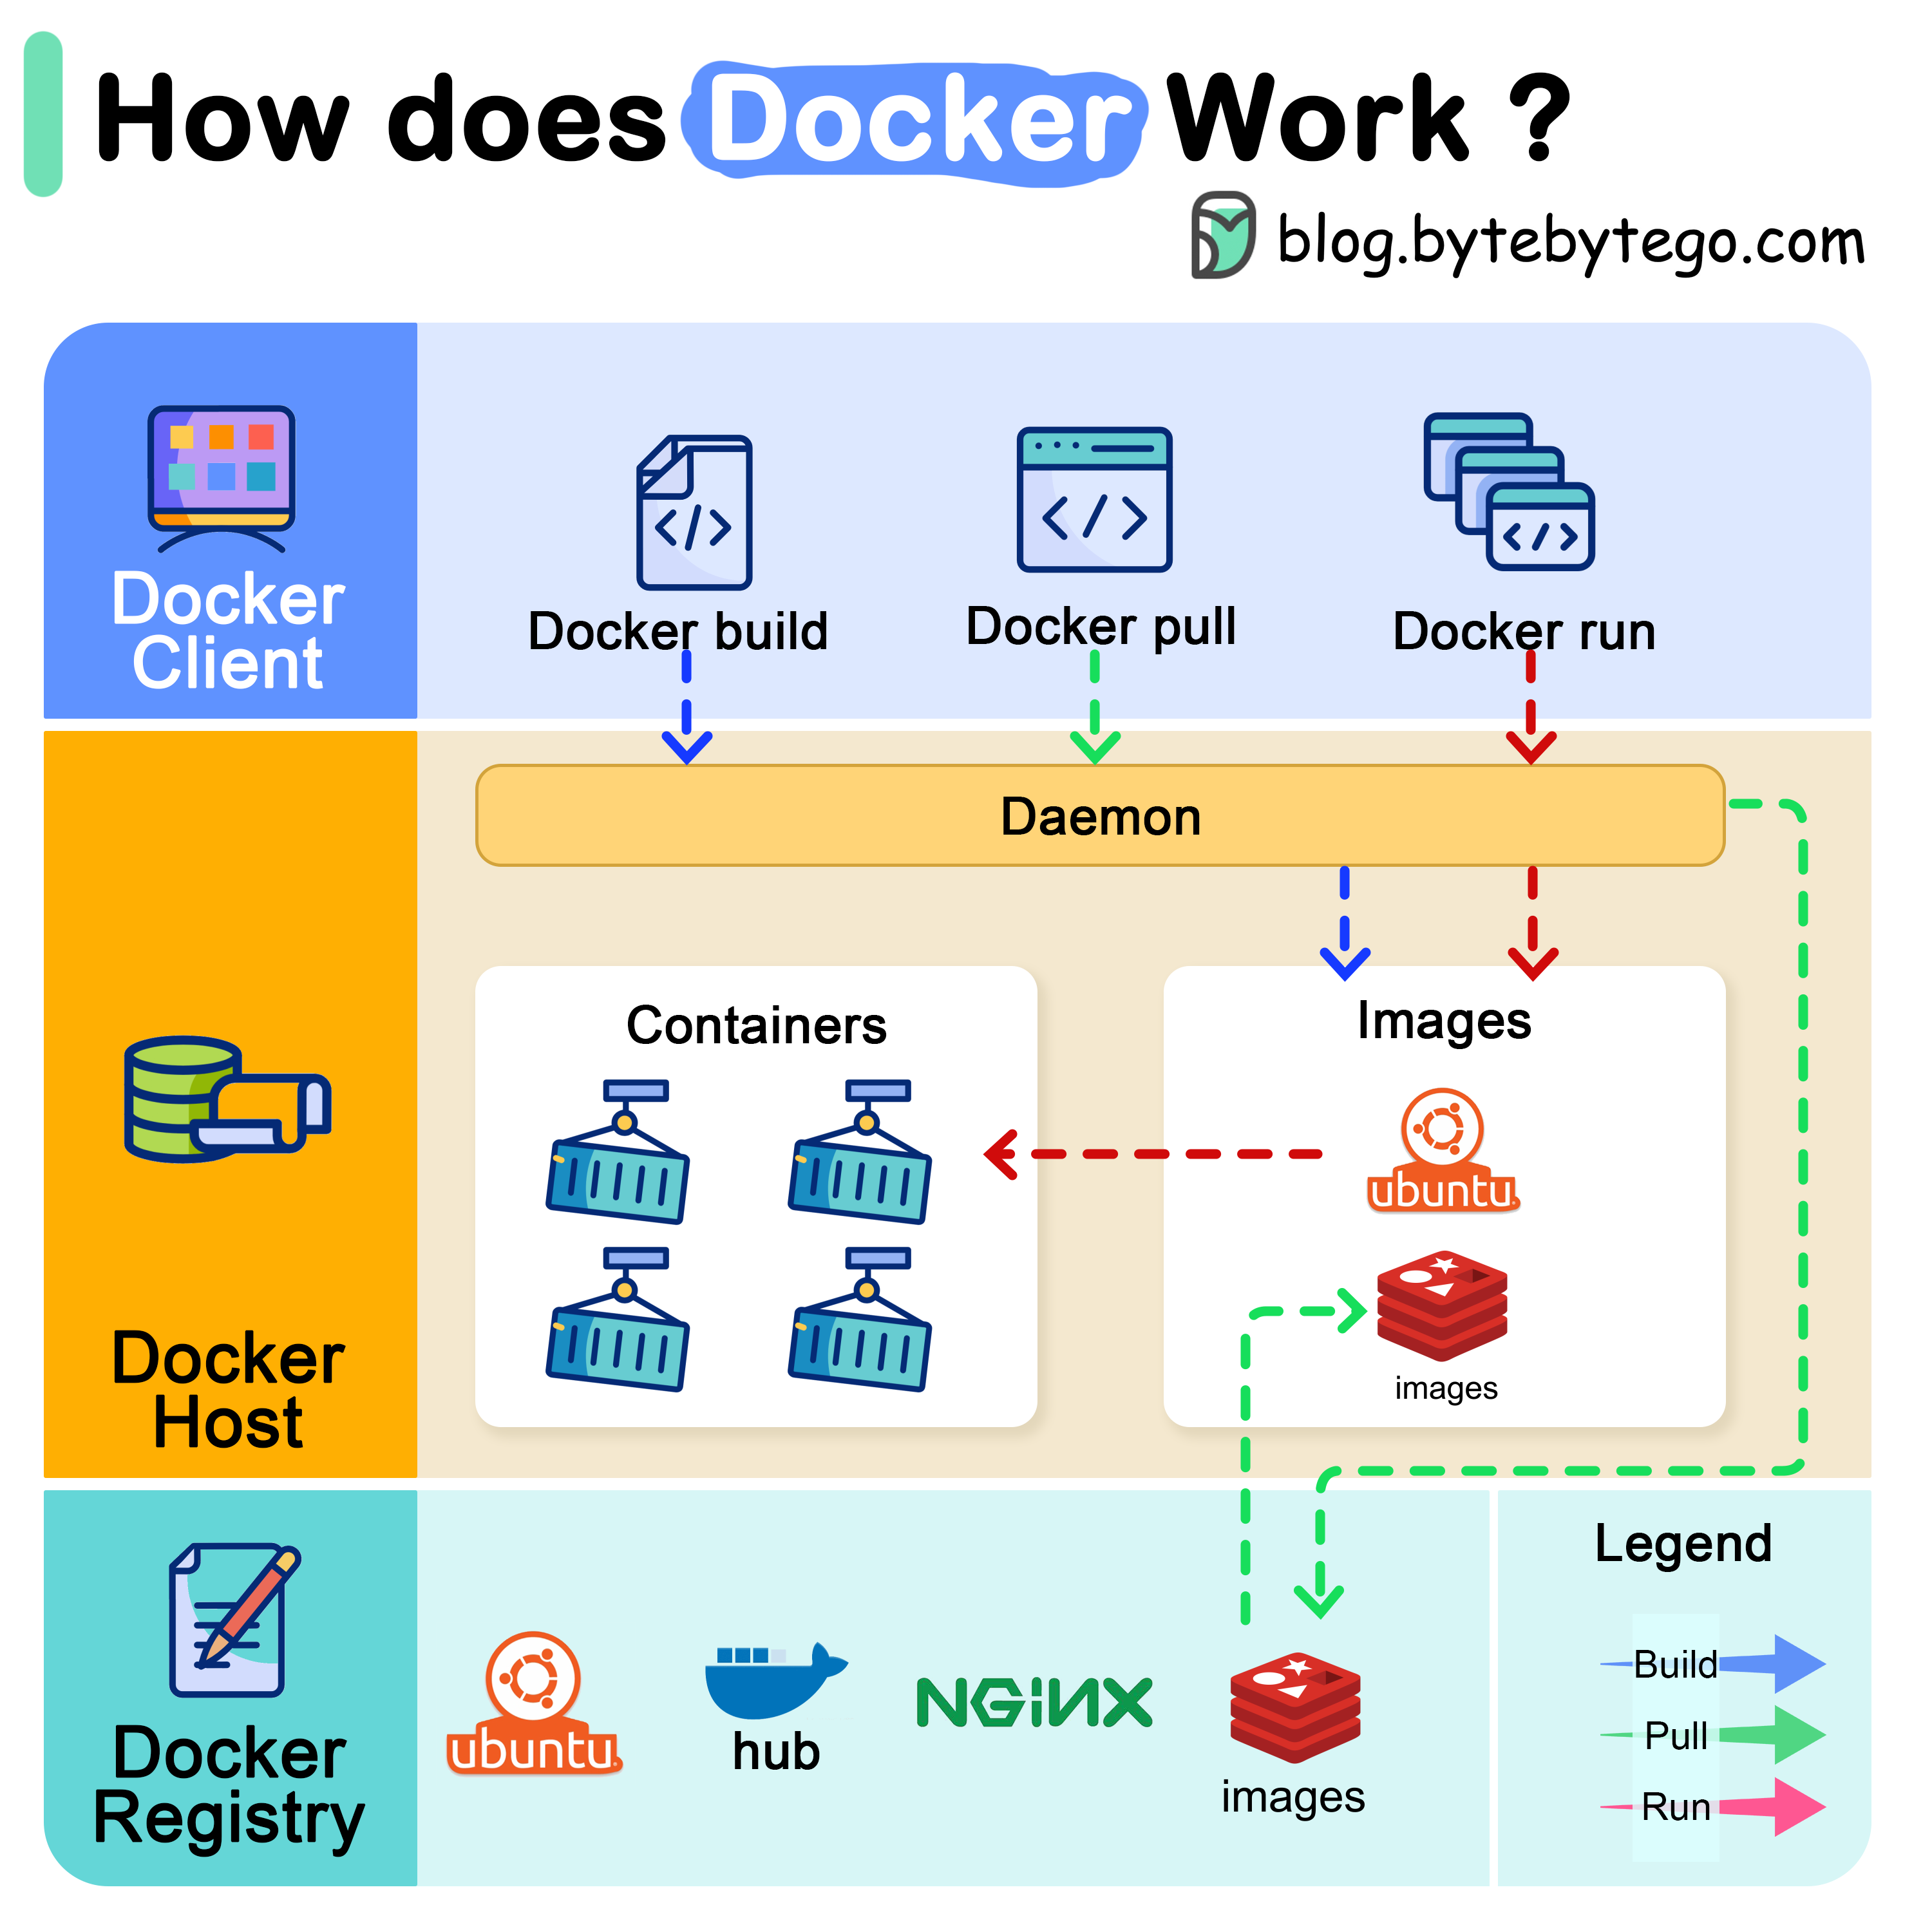
\includegraphics[width=0.85\textwidth]{pics/0414-how-does-docker-work.png}
    \caption{Grundlegende Architektur von Docker}
    \label{fig:docker-architecture}
\end{figure}